\subsection{Echo State Networks}

\begin{figure}[htp]
  \centering
  \subfloat[Training Flow]{
    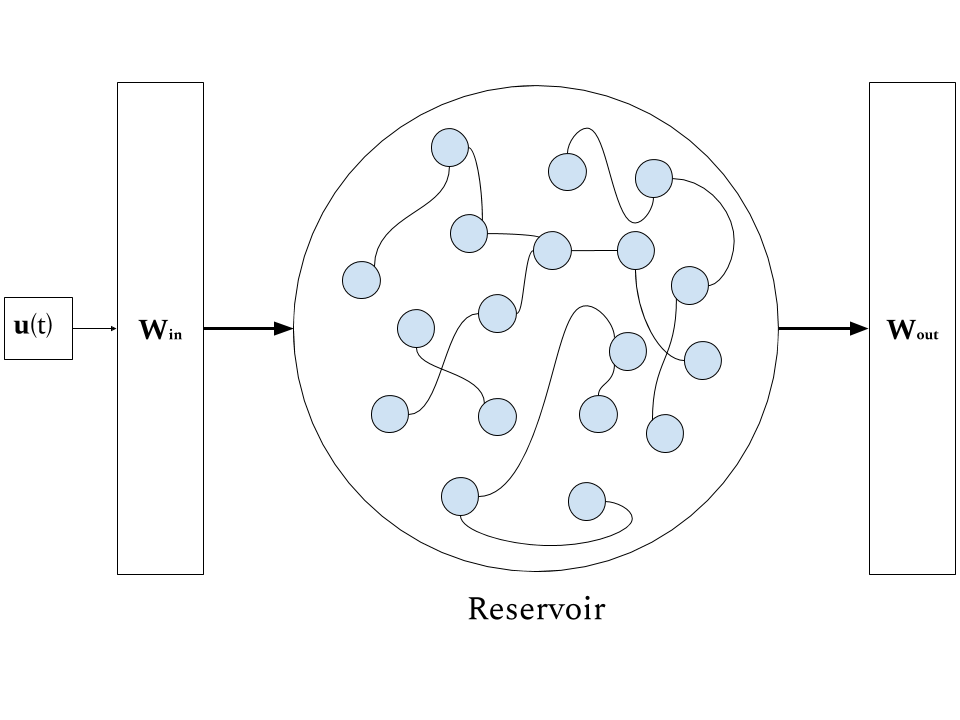
\includegraphics[clip, width=0.85\columnwidth]{reservoir_training.png}
  }


  \subfloat[Predicting Flow]{
    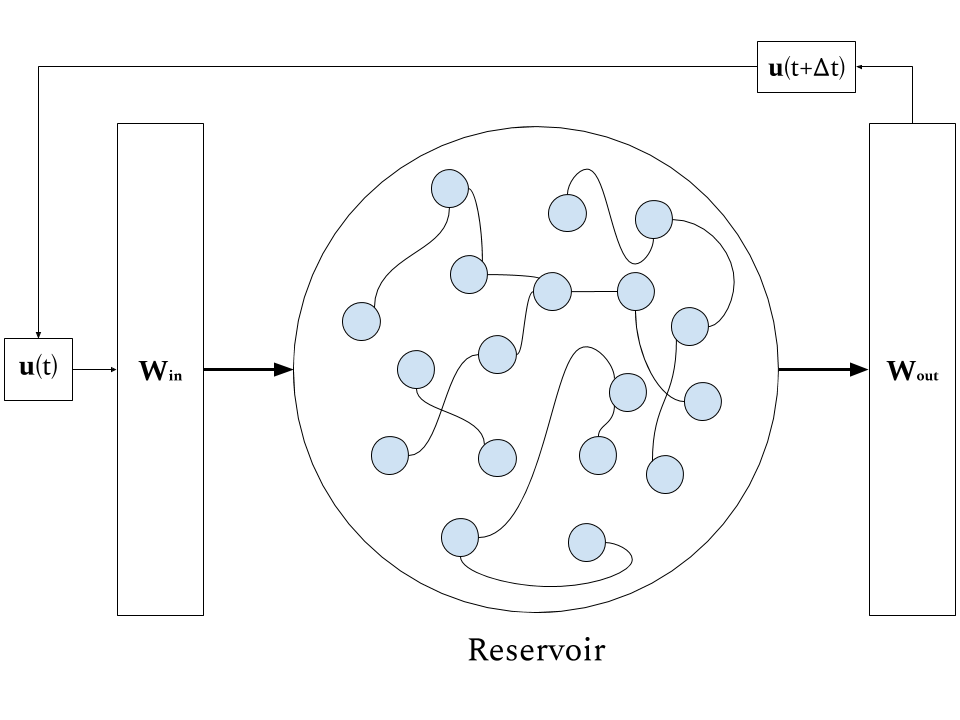
\includegraphics[clip, width=0.85\columnwidth]{reservoir_predicting.png}
  }
  \caption{(a) Shows the behavior of an \gls{esn} during the training phase. (b) Shows \gls{esn} behavior during the predicting phase. The output $u(t+\Delta t)$ is used as the next input value. }
  \label{fig:reservoir_graph}
\end{figure}

An \gls{esn}, sometimes called a ``reservoir
computer,''\cite{pathak_using_2017, pathak_model-free_2018, vlachas_backpropagation_2020} is a type of recurrent
neural network that replaces the many hidden layers of a conventional feed-forward
neural network with a reservoir that is:
\begin{enumerate}
  \item sparse,
  \item connected by uniformly random weights, centered at zero,
  \item and large (i.e. has many neurons).
\end{enumerate}

The reservoir is therefore a randomly instantiated adjacency matrix,
\textit{\textbf{W}}, of size $N \times N$. The input vector, $U(t)$, of
$K$ units is mapped onto the reservoir by an input matrix,
 $W^{in}$ of size $N \times K$. The activation states of the reservoir are calculated by
 \begin{align}
   x(t) &= \tanh \left(W^{in}\cdot U(t) + \mathbf{W}x(t-1)\right)
 \end{align}
 Where $x(t)$ is the collection of reservoir activations \cite{shi_energy_2016, pathak_model-free_2018, lukosevicius_practical_2012}.
 The output is read by an output weight matrix,
 $W^{out}$.
 \begin{align}
   U(t+\Delta t) &= \left(W^{out}\right)^T\cdot x(t)
 \end{align}
 In the training phase, the output, $U(t+\Delta t)$, is
 discarded and the next training input is passed to the network. During the
 prediction phase, the output is kept and used as the next input. Figure \ref{fig:reservoir_graph} illustrates this behavior. The speed of \glspl{esn} is owed
 to this structure--- only $W^{out}$ has tunable weights. Everything else is
 fixed. In this work, we adapted the open source Python package \texttt{pyESN} \cite{korndorfer_pyesn_2015} to construct and train the network.

 \subsection{Hyper-Parameter Optimization}

 \glspl{esn} are fast because the hidden layer in a conventional feed-forward neural network is replaced by a large reservoir that does not require training.
 The trade off is that \glspl{esn} are sensitive to various hyper-parameters
 that need to be optimized \cite{lukosevicius_practical_2012}. These hyper-parameters are summarized in Table \ref{tab:parameters}. The spectral radius ($\rho$) should satisfy the ``echo state property'' which means that
 previous reservoir activations have a decaying influence on future states. This
 is usually guaranteed for $\rho < 1$, but is not a requirement
 \cite{lukosevicius_practical_2012}.
 \begin{table*}[h]
   \centering
   \caption{Description of Model Hyper-Parameters}
   \begin{tabular}{c|c|c}
     \hline
     Hyper-parameter & Purpose & Tested Values\\
     \hline
     \texttt{noise} & Neuron regularization & [0.0001, 0.0003, 0.0007, 0.001, \\
     &&0.003, 0.005, 0.007, 0.01]\\
     $\rho$ & Spectral radius & [0.5, 0.7, 0.9, 1, 1.1, \\
     &&1.2, 1.3, 1.5]\\
     $N$ & Size of reservoir, \textbf{W} & [600, 800, 1000, 1500, 2000, \\
     &&2500, 3000, 4000]\\
     \texttt{sparsity} & The density of connections in \textbf{W}& [0.005, 0.01, 0.03, 0.05, \\
     &&0.1, 0.12, 0.15, 0.2]\\
     Training Length & Size of the training set before prediction & $L \in$ [5000, 25000], step size = 300
   \end{tabular}
   \label{tab:parameters}
 \end{table*}

 We optimize the hyper-parameters by performing a grid search over the test
 values specified in Table \ref{tab:parameters}. We took the following
 optimization steps for each prediction task:
 \begin{enumerate}
   \item Select a hyper-parameter or pair of parameters.
   \item Generate \gls{esn} prediction with the specified parameters.
   \item Calculate and record the root mean squared error (RMSE).
   \item Continue until last entry in the parameter set is reached.
   \item Set the network parameters to hyper-parameter value that minimizes the
   RMSE.
 \end{enumerate}
 This algorithm generates an error surface where the coordinates of the absolute
 minimum correspond to the indices of values in the hyper-parameter test sets
 that minimized the RMSE. Figure \ref{fig:rhoxnoise-demand04} shows an example
 heatmap that optimized the spectral radius and noise hyperparameters for the 4-hour
 ahead demand forecast and illustrates the sensitivity of \glspl{esn} to
 hyperparameter values.

 \begin{figure}[h]
   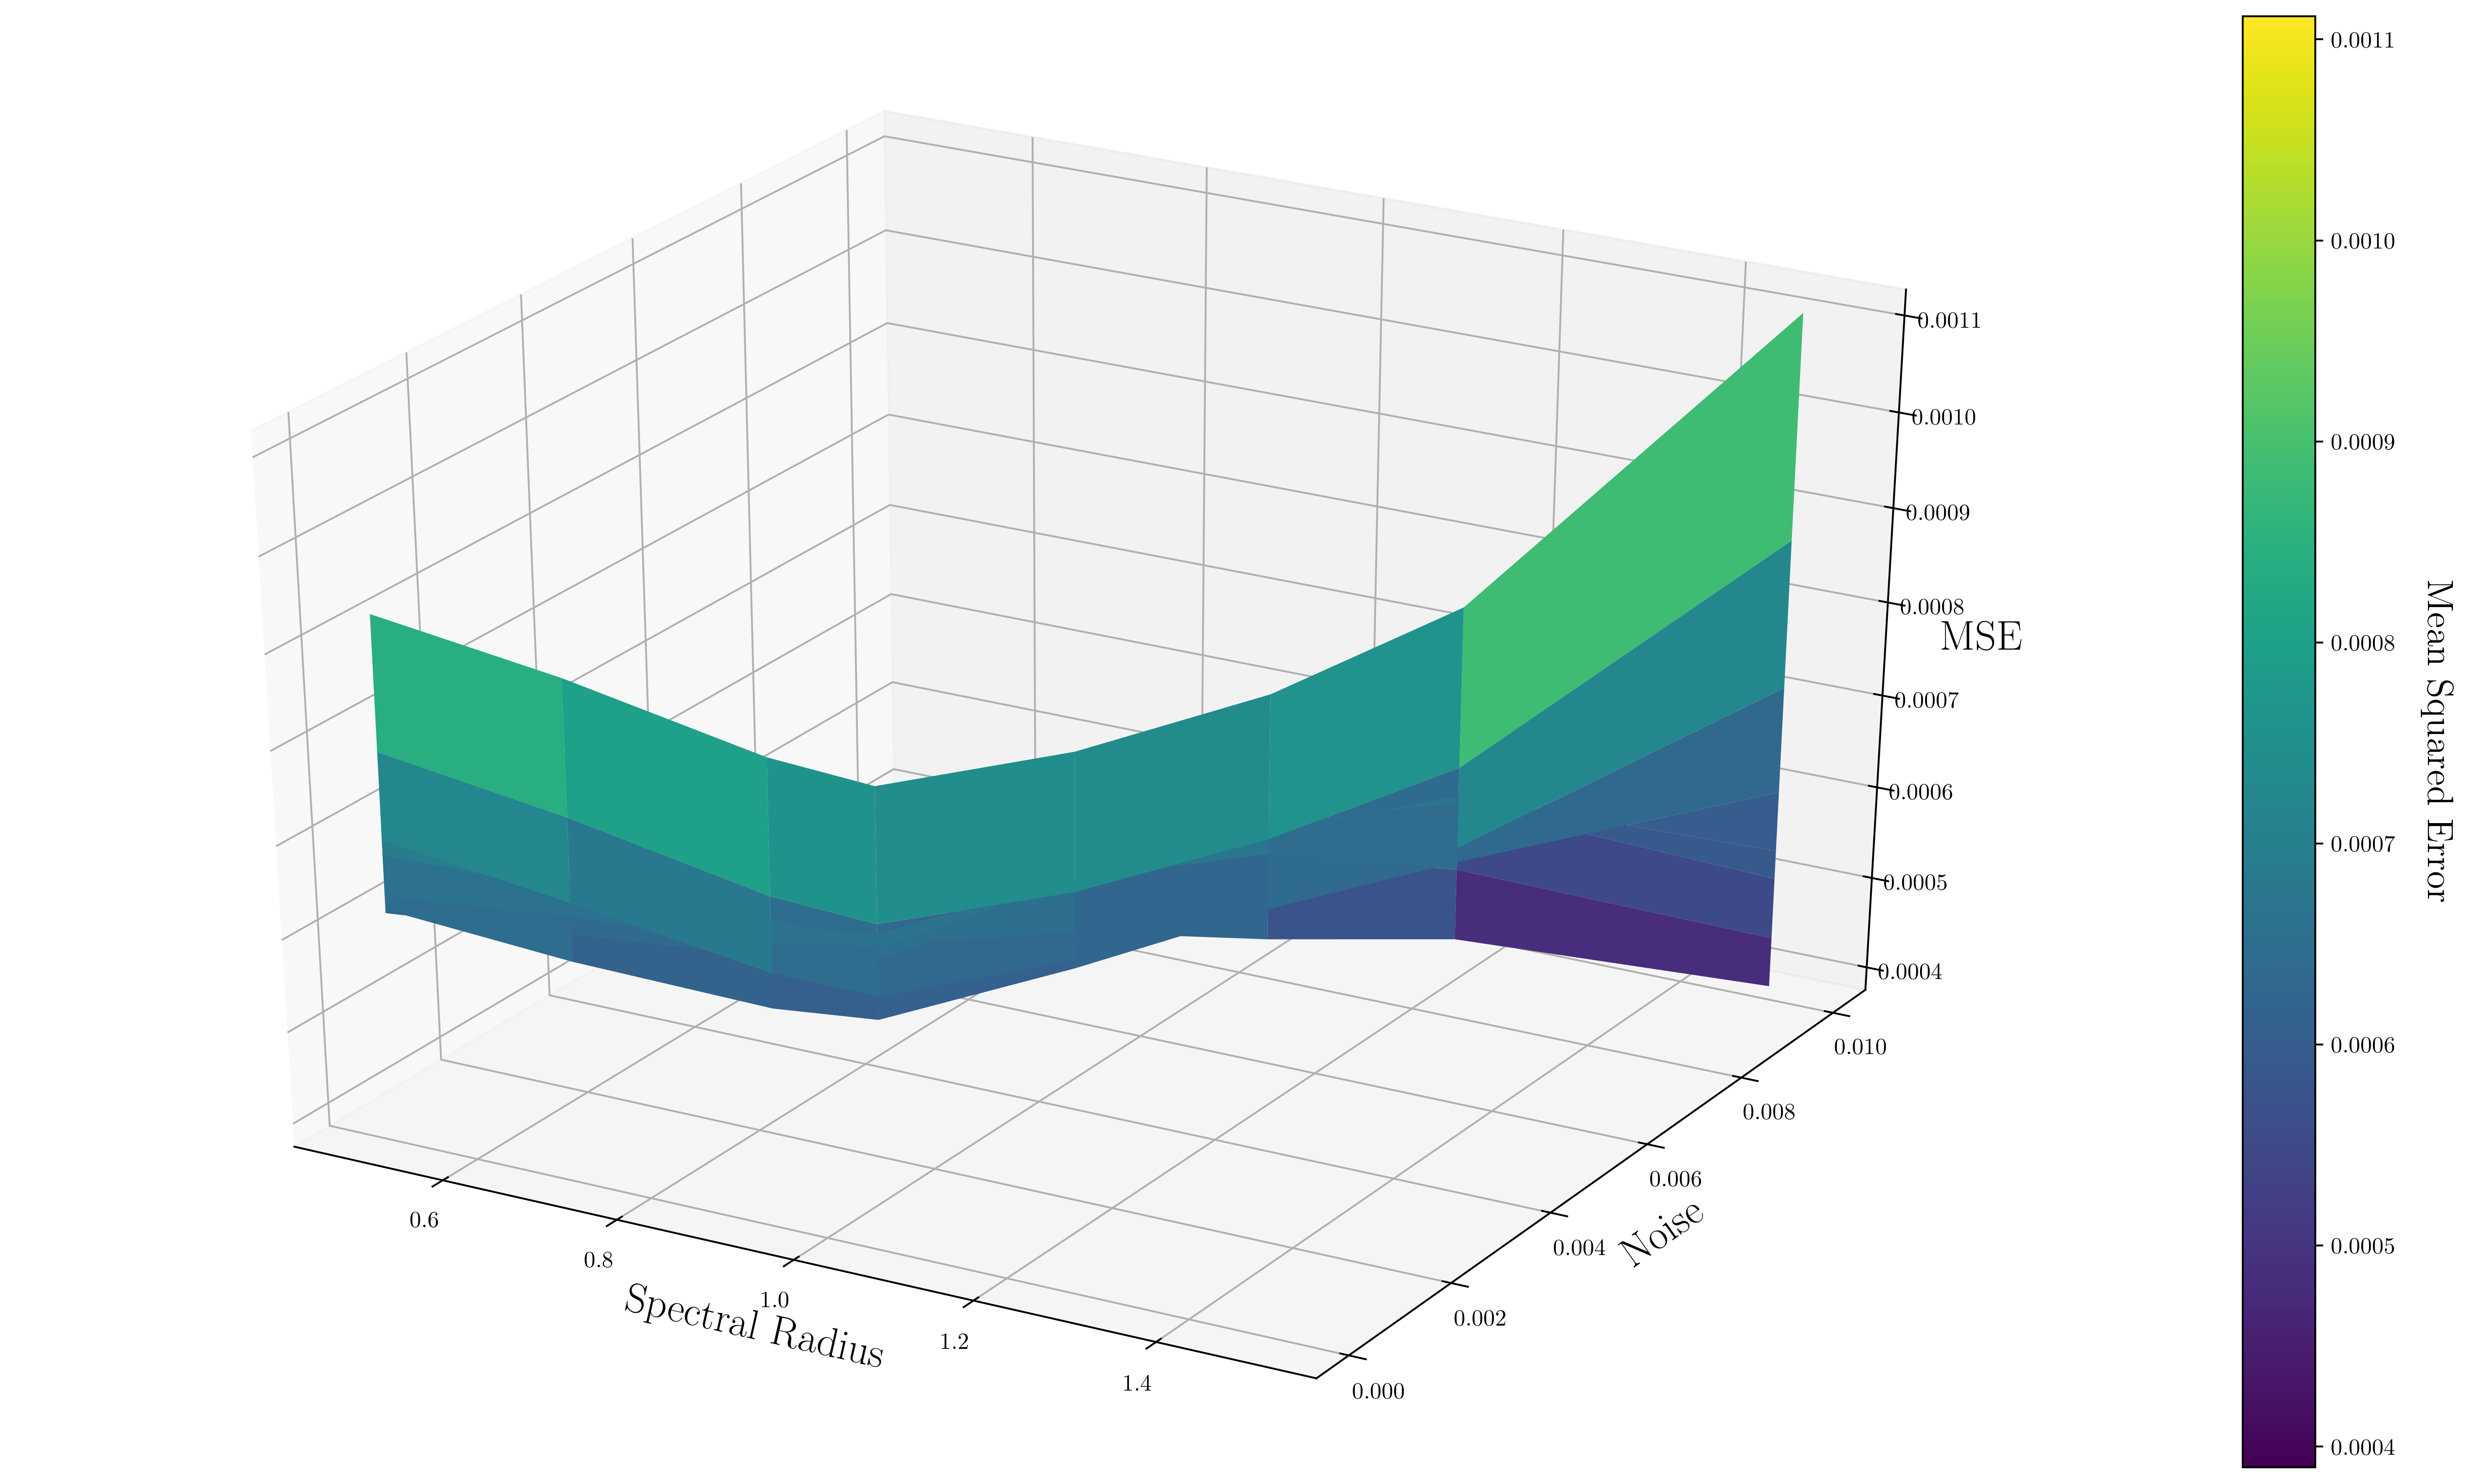
\includegraphics[width=\columnwidth]{./images/04_demand_rho_noise_loss.png}
   % \input{./images/04_wind_elevation_rho_noise_loss-img0.png}
   \caption{An example heatmap of the RMSE for 4-hour ahead demand prediction with different combinations of spectral radius, $\rho$, and noise.}
   \label{fig:rhoxnoise-demand04}
 \end{figure}

 \subsection{Prediction Tasks}

We first performed a benchmarking task by making a prediction for the Lorenz
1963 model \cite{lorenz_deterministic_1963}. Then, we optimized predictions for
univariate time-series
representing total demand, solar energy, and wind energy 4-hours ahead and
48-hours ahead. Finally, we repeated those same six tasks with an additional
predictor. The tasks are summarized in Table \ref{tab:tasks}.

\begin{table*}[h]
  \centering
  \caption{Summary of Prediction Tasks}
  \label{tab:tasks}
  \begin{tabular}{c|c|c}
    \hline
    Target & Future & Additional Predictor\\
    \hline
    && None \\
    Total Demand && Solar Elevation\\
    &4-hours ahead& Humidity\\
    Solar Energy && Pressure\\
    &48-hours ahead& Wet Bulb Temp.\\
    Wind Energy && Dry Bulb Temp.\\
    && Wind Speed\\
  \end{tabular}\\[-1.4pt]%

\end{table*}
